\documentclass[a4paper, 11pt]{report}
%package import
\usepackage{verbatim}
\usepackage[utf8]{inputenc}
\usepackage{listings}
\usepackage{fancyhdr}
\usepackage[hmargin=3cm]{geometry}
\usepackage[spanish]{babel}
\usepackage{ifthen}
\usepackage{graphicx}
\usepackage{tikz}
    \usetikzlibrary{positioning}
\usepackage{algpseudocode}
\usepackage{algorithm}
\usepackage{amsfonts}
%NewCommands
\newcommand{\HRule}[1]{\rule{\linewidth}{#1}}

\newcommand{\DrawGraph}[5]{

    \begin{scope}[#4]
    \foreach \pos/\nodo in {{(0,0)/1}, {(2,1)/2}, {(4,1)/3}, {(0,2)/4}, {(3,0)/5}, {(2,-1)/6}, {(4,-1)/7}}
        \node[vertex] (#3\nodo) at \pos {\nodo};

    \foreach \start/\end in {1/4, 1/2, 1/6,2/5,2/3,2/6,5/7,3/7,4/2,6/7}
        \path[edge,#5] (#3\start) -- (#3\end);

    \foreach \nodo in {#1}
        \node[selected vertex] at (#3\nodo) {\nodo};
        

    \begin{pgfonlayer}{background}
        \foreach \start/\end in {#2}
            \path[selected edge,#5] (#3\start) -- (#3\end);
    \end{pgfonlayer}
    \end{scope}
}

\newcommand{\DrawWGraph}[5]{

    \begin{scope}[#4]
    \foreach \pos/\nodo in {{(0,0)/1}, {(2,1)/2}, {(4,1)/3}, {(0,2)/4}, {(3,0)/5}, {(2,-1)/6}, {(4,-1)/7}}
        \node[vertex] (#3\nodo) at \pos {\nodo};

    \foreach \start/\end/\weight in {1/4/5, 1/2/4, 1/6/16,2/5/20,2/3/5,2/6/8,5/7/14,3/7/3,4/2/1,6/7/8}
        \path[edge,#5] (#3\start) --node[weight,midway,fill=white] {$\weight$} (#3\end);

    \foreach \nodo in {#1}
        \node[selected vertex] at (#3\nodo) {\nodo};

    \begin{pgfonlayer}{background}
        \foreach \start/\end in {#2}
            \path[selected edge,#5] (#3\start) -- (#3\end);
    \end{pgfonlayer}
    \end{scope}

}
\newcommand{\DrawEJGraph}[5]{

    \begin{scope}[#4]
    \foreach \pos/\nodo in {{(0,0)/4}, {(0,2.2)/5}, {(1.5,1.7)/7}, {(3,3)/1}, {(3,1)/0}, {(4.5,1.7)/2}, {(4.5,3)/3}, {(7,0)/6}}
        \node[vertex] (#3\nodo) at \pos {\nodo};

    \foreach \start/\end/\weight in {4/5/0.35, 5/7/0.28, 7/1/0.19,7/0/0.16,0/2/0.26,2/3/0.17,2/6/0.40,4/7/0.37,1/5/0.32,0/4/0.38,1/2/0.36,1/3/0.29,2/7/0.34,3/6/0.52,6/0/0.58,6/4/0.93}
        \path[edge,#5] (#3\start) --node[weight,midway,fill=white] {$\weight$} (#3\end);

    \foreach \nodo in {#1}
        \node[selected vertex] at (#3\nodo) {\nodo};

    \begin{pgfonlayer}{background}
        \foreach \start/\end in {#2}
            \path[rojog edge,#5] (#3\start) -- (#3\end);
    \end{pgfonlayer}
    \end{scope}

}
\newcommand{\DrawEJcGraph}[5]{

    \begin{scope}[#5]
    \foreach \pos/\nodo in {{(0,0)/4}, {(0,1.2)/5}, {(1,1)/7}, {(2,2.2)/1}, {(2,0.6)/0}, {(3.4,0.9)/2}, {(3.4,2.2)/3}, {(5,0)/6}}
        \node[vertex] (#3\nodo) at \pos {\nodo};
    \foreach \start/\end in {4/5, 5/7, 7/1,7/0,0/2,2/3,2/6,4/7,1/5,0/4,1/2,1/3,2/7,3/6,6/0,6/4}
        \path[edge,#5] (#3\start) -- (#3\end);

    \foreach \nodo in {#1}
        \node[selected vertex] at (#3\nodo) {\nodo};

    \begin{pgfonlayer}{background}%rojo delgado
        \foreach \start/\end in {#2}
            \path[rojod edge,#5] (#3\start) -- (#3\end);
    \end{pgfonlayer}
    \begin{pgfonlayer}{background}%rojo grueso
        \foreach \start/\end in {#3}
            \path[rojog edge,#5] (#3\start) -- (#3\end);
    \end{pgfonlayer}
    \begin{pgfonlayer}{background}%azul
        \foreach \start/\end in {#4}
            \path[azul edge,#5] (#3\start) -- (#3\end);
    \end{pgfonlayer}
    \end{scope}

}







\newcommand{\DrawArrow}[1]{
    \begin{scope}[scale=0.5,#1]
        \filldraw[arrow] (0,0) -- (2,0) -- +(270:0.5) -- (3,0.5) -- (2,1.5) -- +(270:0.5) -- (0,1) -- cycle;
    \end{scope}
}

\newcommand{\DrawAdjMat}{
	\node[nodo] (1) at (0,0) {$1$};
    \node[nodo] (2) [below = 0pt of 1] {2};
    \node[nodo] (3) [below = 0pt of 2] {3};
    \node[nodo] (4) [below = 0pt of 3] {4};
	\node[cell] (primero) [right = 0pt of 1] {T};
    \node[cell] (segundo) [right =0pt of primero] {T};
    \node[cell] (tercero) [right = 0pt of segundo] {F};
    \node[cell] (cuarto) [right = 0pt of tercero] {T};
    \node[nodo] (1c) [above = 0pt of primero] {1};
	\node[nodo] (2c) [above = 0pt of segundo] {2};
   	\node[nodo] (3c) [above = 0pt of tercero] {3};
    \node[nodo] (4c) [right = 0pt of 3c] {4};
   	\node[cell] (primero2) [right = 0pt of 2] {T};
    \node[cell] (segundo2) [right =0pt of primero2] {T};
    \node[cell] (tercero2) [right = 0pt of segundo2] {T};
    \node[cell] (cuarto2) [right = 0pt of tercero2] {F};
   	\node[cell] (primero3) [right = 0pt of 3] {F};
    \node[cell] (segundo3) [right =0pt of primero3] {T};
    \node[cell] (tercero3) [right = 0pt of segundo3] {T};
    \node[cell] (cuarto3) [right = 0pt of tercero3] {T};
	\node[cell] (primero4) [right = 0pt of 4] {T};
    \node[cell] (segundo4) [right =0pt of primero4] {F};
    \node[cell] (tercero4) [right = 0pt of segundo4] {T};
    \node[cell] (cuarto4) [right = 0pt of tercero4] {T};

	\begin{scope}[xshift = 3cm, yshift = -1mm,scale = 1.5]
    \foreach \pos/\nodo in {{(0,0)/1}, {(1,0)/2}, {(0,-1)/3}, {(1,-1)/4}}
        \node[vertex_adjMat] (\nodo) at \pos {\nodo};

    \foreach \start/\end in {1/2,1/4,4/3,2/3}
        \path[edge] (\start) -- (\end);
    \end{scope}
}

\newcommand{\DrawAdjList}{
    \node[nodo] (1) at (0,0) {$1$};
    \node[nodo] (2) [below = 0pt of 1] {2};
    \node[nodo] (3) [below = 0pt of 2] {3};
    \node[nodo] (4) [below = 0pt of 3] {4};
	\node[cell] (primero) [right = 0pt of 1] {2};
    \node[cell] (segundo) [right =0pt of primero] {4};
   	\node[cell] (primero2) [right = 0pt of 2] {1};
    \node[cell] (segundo2) [right =0pt of primero2] {3};
   	\node[cell] (primero3) [right = 0pt of 3] {2};
    \node[cell] (segundo3) [right =0pt of primero3] {4};
	\node[cell] (primero4) [right = 0pt of 4] {1};
    \node[cell] (segundo4) [right =0pt of primero4] {3};

	\begin{scope}[xshift = 3cm, yshift = -1mm,scale = 1.5]
    \foreach \pos/\nodo in {{(0,0)/1}, {(1,0)/2}, {(0,-1)/3}, {(1,-1)/4}}
        \node[vertex_adjMat] (\nodo) at \pos {\nodo};

    \foreach \start/\end in {1/2,1/4,4/3,2/3}
        \path[edge] (\start) -- (\end);
    \end{scope}
    }

\newcommand{\Deactivate}{\shorthandoff{<>."}}
\newcommand{\Activate}{\shorthandon{<>."}}
%Changing space between paragraphs
\setlength{\parskip}{2mm}

%Setting up fancy package
\pagestyle{fancy}
\setlength{\headheight}{15.2pt}
\renewcommand{\chaptermark}[1]{ \markboth{#1}{} }
\renewcommand{\sectionmark}[1]{ \markright{#1}{} }
\fancyhf{}

\fancyhead[C]{
    \footnotesize
    \itshape
    IE-0217% Estructuras Abstractas de Datos y Algoritmos para Ingenier\'ia
    }
 
\fancyhead[L]{
    \footnotesize
    \itshape
    Librer\'ia de Grafos para C++
    }
\fancyhead[R]{
    \footnotesize
    \itshape
    \ifthenelse{\isodd{\value{page}}}{Prof. Francisco Siles Canales}{\rightmark}
    }

\fancyfoot[R]{\thepage}


\begin{document}
%Tikz styles definitions
\tikzstyle{vertex_adjMat}=[circle,fill=blue!25,minimum size=10pt,inner sep=2pt,font = \small]
\tikzstyle{cell} = [shape=rectangle,minimum size=15pt, inner sep=0pt,draw=black!50,fill=white, font=\scriptsize]
\tikzstyle{nodo} = [shape=rectangle,minimum size=15pt, inner sep=0pt,fill=white, font=\footnotesize]

\tikzstyle{vertex}=[circle,fill=blue!25,minimum size=10pt,inner sep=0pt,font = \tiny]
\tikzstyle{selected vertex} = [vertex, fill=red!24]
\tikzstyle{edge} = [draw,thick,-]
\tikzstyle{weight} = [font=\scriptsize]
\tikzstyle{selected edge} = [draw,line width=3pt,-,red!50]
\tikzstyle{ignored edge} = [draw,line width=3pt,-,black!20]
\tikzstyle{rojod edge} = [draw,line width=2pt,-,red!50]
\tikzstyle{rojog edge} = [draw,line width=4pt,-,red!70]
\tikzstyle{azul edge} = [draw,line width=4pt,-,blue!50]
\tikzstyle{arrow} = [fill=red!80, draw = black!20]
\pgfdeclarelayer{background}
\pgfsetlayers{background,main}

%Creating Title
\begin{titlepage}
    \begin{center}
       %ordenar los archivos \includegraphics[width=0.4\textwidth]{logo-eie.jpg}\\[1.5cm]
        \HRule{0.5mm}\\[0.12cm]
        \textsc{\huge Librer\'ia de Grafos para C++}\\[0.2cm]
        \HRule{0.8mm}\\[1.7cm]
        \begin{flushright}
        \begin{tabular}{l c}
            Hugo Z\'u\~niga C. & A96988 \\
            Ernesto C\'espedes M. & AXXXXX \\
            Diego \'Alvarez A. & AXXXXX \\
        \end{tabular}
        \end{flushright}

    \end{center}
\end{titlepage}
%*/*/*/*/*/*/*/*/*/*//*/*/*/*/*/*/*/*/*/*/*/*/*/*/*/*/*/*/*/*/*/*
%                   Documento
%*/*/*/*/*/*/*/*/*/*//*/*/*/*/*/*/*/*/*/*/*/*/*/*/*/*/*/*/*/*/*

\chapter{Marco Te\'orico}
\section{Introducci\'on a los Grafos}
Un grafo es la representaci\'on abstracta de un conjunto de objetos, los cuales est\'an conectados a trav\'es de enlaces. Los objetos interconectados se representan mediante una estructura denominada v\'ertice y a los enlaces se les denomina bordes. La representaci\'on  gr\'afica de un grafo se hace mediante un conjunto de puntos (v\'ertices) unidos por un conjunto de l\'ineas que representan los bordes, un ejemplo de esto se observa en la figura \ref{EjGrafo}.

\begin{figure}[!h]
    \centering
    \begin{tikzpicture}
        \DrawGraph{}{}{a}{}{}
    \end{tikzpicture}
    \caption{Representaci\'on Gr\'afica de un Grafo}
    \label{EjGrafo}
\end{figure}

Los grafos son estructuras de datos que tienen aplicaciones en muchas \'areas del desarrollo humano, algunas de ellas son:

\begin{itemize}
    \item \emph{Desarrollo de Circuitos Integrados:} Los circuitos electr\'onicos constan de una gran cantidad de componentes, los cuales est\'an interconectados mediante l\'ineas de metal. Debido a la complexidad de los dise\~nos es necesario contar con una plataforma la cual permita hacer solicitudes sobre la interconexi\'on de los componentes.
    \item \emph{Transacciones Comerciales:} Las instituciones financieras compran y venden acciones en la bolsa. En este caso el grafo permite representar la transferencia de dinero y bienes entre instituciones o instituciones y compradores.
    \item \emph{Redes de Computadoras:} Las redes de computadoras consisten de un conjunto de computadoras interconectadas, las cuales env\'ian y reciben mensajes de varios tipos. En este caso el grafo representa los nodos del sistema y las v\'ias de comunicaci\'on que hay entre ellas. 
\end{itemize}

\subsection{Tipos de Grafos}
Dentro del sistema de grafos existen diversas subclasificaciones, las cuales representan las distintas estructuras que se pueden obtener con el objetivo de representar las relaciones entre los objetos. Las clasificaciones en las cuales se basa este proyecto son:

\begin{itemize}
    \item Grafos no Dirigidos
    \item Grafos Dirigidos
    \item Grafos con Peso
\end{itemize}

\subsubsection{Grafos no Dirigidos}
Los grafos no dirigidos son estruturas de datos que representan un sistema en el cual los enlaces permiten la conexi\'on bidireccional entre los v\'ertices, la representaci\'on gr\'afica de este tipo se observa en la figura \ref{EjGrafo}. Asimismo dentr de la estructura de datos, existen subestructuras que permiten encontrar propiedades importantes de los grafos.

La primera de estas subestructuras es el <<path>> o camino, el cual es una secuencia de v\'ertices conectados por enlaces. De esta manera existen caminos simples, los cuales cuentan con todos los v\'ertices distintos y existen caminos c\'iclicos, en los cuales se repite el primer y \'ultimo v\'ertice. Esta definici\'on es una de las m\'as importantes en la teor\'ia de grafos, ya que uno de los par\'ametros de mayor inter\'es de un grafo es la capacidad de encontrar un camino que interconecte dos v\'ertices y determinar si es el \'optimo.

Otra estructura importante relacionada con los grafos es el \'arbol, el cual es un subgrafo que contiene todos los v\'ertices pertenecientes al grafo. La importancia de esta estructura radica en su utilizaci\'on en los algoritmos de procesamiento de grafos, esta representaci\'on permite obtener informaci\'on importante acerca de la conectividad y estructura del grafo.

\subsubsection{Grafos Dirigidos}
La singularidad que tienen los grafos dirigidos es que los enlaces entre los v\'ertices son unidireccionales a diferencia de los grafos no dirigidos. Esto implica que los enlaces pueden ser atravesados en una direcci\'on \'unicamente.

De esta manera existen tambi\'en la definici\'on de camino simple y camino c\'iclico para los grafos dirigidos. La diferencia principal radica en la limitaci\'on de que el hecho de que exista un camino que comunique dos v\'ertices en una direcci\'on no implica que exista un camino que los comunique de manera inversa.

\begin{figure}[!h]
    \centering
    \Deactivate
    \begin{tikzpicture}
        \DrawGraph{}{}{a}{}{->}
    \end{tikzpicture}
    \Activate
    \caption{Representaci\'on Gr\'afica del Grafo Dirigido}
    \label{EjGrafoDirigido}
\end{figure}

\subsubsection{Grafos con Peso}
En realidad los grafos con peso se pueden basar en cualquiera de las dos estruturas discutidas anteriormente, la diferencia principal es que se le agrega informaci\'on a los enlaces, de manera que se puedan adaptar al modelado de sistemas m\'as amplios.

\begin{figure}[!h]
    \centering
    \begin{tikzpicture}
        \DrawWGraph{}{}{a}{}{}
    \end{tikzpicture}
    \caption{Representaci\'on Gr\'afica del Grafo con Peso}
    \label{EjGrafoPeso}
\end{figure}

\subsection{Estructura de Datos}
Dentro del estudio de la eficiencia de los algoritmos, se toman en cuenta dos par\'ametros el tiempo y espacio de ejecuci\'on. El primero hace referencia al tiempo que toma completar el procesamiento del algoritmo, mientras que el segundo trata sobre la cantidad de espacio que ocupan todas las estructuras y funciones que son necesarias para la ejecuci\'on del algoritmo.

En consideraci\'on de estos par\'ametros es importante determinar una estructura de datos para la representaci\'on de grafos, la cual permita obtener la flexibilidad necesaria de manera que se optimicen tanto el tiempo de ejecuci\'on de los algoritmos como el espacio de almacenamiento. Para alcanzar este fin se estudi\'o tres propuestas diferentes.

\begin{itemize}
    \item Matriz de Adyacencia
    \item Arreglo de Enlaces
    \item Lista de Adyacencias
\end{itemize} 

\subsubsection{Matriz de Adyacencia}

La matriz de adyacencia es una configuraci\'on, en la cual el grafo se representa mediante una matriz de N filas y N columnas, donde N representa la cantidad de v\'ertices presentes en el grafo. Para reprecentar los enlaces entre v\'ertices, se asigna un valor booleano a la celda representado por la fila y la columna de los nodos conectados, as\'i por ejemplo el siguiente es un ejemplo de una matriz de adyacencia de 4 v\'ertices. 

\begin{figure}[!h]
	\centering
	\begin{tikzpicture}
		\DrawAdjMat
	\end{tikzpicture}
    \caption{Representaci\'on de un grafo mediante una matriz de adyacencia}
    \label{AdjMat}
\end{figure}

La ventaja de la configuraci\'on es que permite una r\'apida inserci\'on de nuevas conexiones, sin embargo el espacio que ocupa es el cuadrado de la cantidad de v\'ertices, por lo cual esta opci\'on es descartable.

\subsubsection{Arreglo de Enlaces}
El arreglo de enlaces es un sistema, el cual parte de un tipo de dato denominado Enlace, el cual contiene dos variables instanciadas (los v\'ertices conectados). De esta manera es sencillo crear nuevas uniones, sin embargo el tratamiento de los algoritmos para este tipo de organizaci\'on es significativamente m\'as dif\'icil, ya que hay que revisar todos las instancias de <<Enlace>> para poder extraer informaci\'on relevante del grafo.

\subsubsection{Lista de Adyacencias}
La lista de adyacencias es una configuraci\'on en la cual se crea una lista de todos los v\'ertices que est\'an conectados a un nodo en particular, adem\'as se crea una lista con los punteros a las listas de adyacencias. Una representaci\'on de una lista de adyacencias se observa en la figura \ref{ListAdj}

\begin{figure}[!h]
    \centering
    \begin{tikzpicture}
        \DrawAdjList
    \end{tikzpicture}
    \caption{Representaci\'on de la lista de adyacencias}
    \label{ListAdj}
\end{figure}

Esta estructura tiene una complejidad espacial de \emph{E+V}, lo cual es menor que cualquiera de las dos opciones presentadas anteriormente, asimismo el tiempo computacional de procesamiento debe ser menor debido a que en caso de que se desee iterar a trav\'es delos nodos adyacentes, s\'olo se debe revisar los nodos adyacentes, lo cual reduce el tiempo de procesamiento. 

\section{Algoritmos de Procesamiento de Grafos}

\subsection{Algoritmos b\'asicos:}
\subsubsection{Depth First Search}
El algoritmo depth fist search es un algoritmo recursivo, en el cual se siguen los enlaces en el algoritmo para ir revelando nuevos v\'ertices que est\'an directamente conectados a un v\'ertice origen. Este algoritmo tiene diversas aplicaciones, como la determinaci\'on de que haya un camino que conecte dos v\'ertices distintos, tambi\'en se puede utilizar para separar subgrafos en un grafo determinado. 

Dependiendo de la aplicaci\'on la implementaci\'on del depth first search se lleva a cabo de una manera diferente. Para el caso m\'as sencillo que es para determinar conectividad se utiliza una lista para indicar si el v\'ertice fue visitado anteriormente o no. Con base en esta lista se puede determinar si el sistema est\'a conectado (Todos los v\'ertices fueron visitados) o no. Un ejemplo del algoritmo de Depth First Search se presenta a continuaci\'on.

\begin{figure}[!h]
    \centering
    \begin{tikzpicture}
        \Deactivate
        \begin{scope}[scale=0.5]
        \DrawGraph{1}{}{a}{}{-}
        \DrawArrow{xshift=9cm,scale=0.4}
        \DrawGraph{1,4}{1/4}{b}{xshift=5.7cm}{-}
        \DrawArrow{xshift=20.2cm,scale=0.4}
        \DrawGraph{1,4,2}{1/4,4/2}{c}{xshift=11.4cm}{-}
        \DrawArrow{xshift=31.4cm,scale=0.4}
        \DrawGraph{1,4,2,3}{1/4,4/2,2/3}{d}{xshift=17.1cm}{-}
        \DrawArrow{xshift=42.8cm,scale=0.4}
        \DrawGraph{1,4,2,3,7}{1/4,4/2,2/3,3/7}{e}{yshift=-4cm}{-}
        \DrawArrow{xshift=9cm,scale=0.4,yshift=-20cm}
        \DrawGraph{1,4,2,3,7,5}{1/4,4/2,2/3,3/7,2/5}{f}{yshift=-4cm,xshift=5.7cm}{-}
        \DrawArrow{xshift=20.2cm,scale=0.4,yshift=-20cm}
        \DrawGraph{1,4,2,3,7,5,6}{1/4,4/2,2/3,3/7,2/5,1/6}{g}{yshift=-4cm,xshift=11.4cm}{-}
        \end{scope}
        \Activate
    \end{tikzpicture}
    \caption{Ejemplo de la aplicaci\'on del DFS en grafos}
    \label{DFSFigure}
\end{figure}

\subsubsection{Breadth First Search}
El algoritmo Breadth First Search se utiliza para analizar todos los v\'ertices de un grafo no dirigido, este algoritmo a diferencia del Depth First Search itera sobre los v\'ertice en orden de nivel desde el origen, esto quiere decir que visita primero los v\'ertices conectados directamente al origen, luego visita los v\'ertices que est\'an conectados a estos y as\'i sucesivamente. Una de las ventajas que tiene el Breadth First Search es que permite obtener un \'Arbol del Camino m\'as corto para un grafo no dirigido. 

La implementaci\'on del algoritmo hace uso de una cola la cual alberga los v\'ertices como deben irse revisando, para esto lo que se hace es que se introducen a la cola los v\'ertices que est\'en conectados al v\'ertice que se est\'a analizando y que no hab\'ian sido visitados anteriormente. El algoritmo en este caso es iterativo y se revisan todos los v\'ertices hasta que la cola est\'e vac\'ia.

\begin{figure}[!h]
    \centering
    \begin{tikzpicture}
        \Deactivate
        \begin{scope}[scale=0.5]
        \DrawGraph{1}{}{a}{}{-}
        \DrawArrow{xshift=9cm,scale=0.4}
        \DrawGraph{1,4}{1/4}{b}{xshift=5.7cm}{-}
        \DrawArrow{xshift=20.2cm,scale=0.4}
        \DrawGraph{1,4,2}{1/4,1/2}{c}{xshift=11.4cm}{-}
        \DrawArrow{xshift=31.4cm,scale=0.4}
        \DrawGraph{1,4,2,6}{1/4,1/2,1/6}{d}{xshift=17.1cm}{-}
        \DrawArrow{xshift=42.8cm,scale=0.4}
        \DrawGraph{1,4,2,6,3}{1/4,1/2,1/6,2/3}{e}{yshift=-4cm}{-}
        \DrawArrow{xshift=9cm,scale=0.4,yshift=-20cm}
        \DrawGraph{1,4,2,6,3,5}{1/4,1/2,1/6,2/3,2/5}{f}{yshift=-4cm,xshift=5.7cm}{-}
        \DrawArrow{xshift=20.2cm,scale=0.4,yshift=-20cm}
        \DrawGraph{1,4,2,6,3,5,7}{1/4,1/2,1/6,2/3,2/5,5/7}{g}{yshift=-4cm,xshift=11.4cm}{-}
        \end{scope}
        \Activate
    \end{tikzpicture}
    \caption{Ejemplo de la aplicaci\'on del BFS en grafos}
    \label{BFSFigure}
\end{figure}

\subsection{Algoritmos enfocados en grafos dirigidos}
Para el procesamiento de grafos dirigidos existen diversos algoritmos que permiten extraer informaci\'on relevante de la estructura. Algunos de estos son:

\begin{itemize}
    \item \textit{Alcanzabilidad}: ¿Es posible llegar desde un v\'ertice a a un v\'ertice b?
    \item \textit{Detecci\'on de Ciclos}: ¿Existe un camino cerrado dentro del grafo?
    \item \textit{Ordenamiento Topol\'ogico}: ¿Se puede ordenar el sistema, de manera que ning\'un v\'ertice que est\'e en la lista de adyacencia de otro se encuentre m\'as a la izquierda que \'este?
\end{itemize}

\subsubsection{Alcanzabilidad}
Para resolver el problema de saber si existe un camino que comunique dos v\'ertices distintos, es necesario utilizar el algoritmo de depth first search, ya que este provee una manera sencilla de construir un \'arbol, el cual incluya todos los nodos alcanzables desde un origen determinado. Con base en lo mencionado en la secci\'on anterior (Algoritmos B\'asicos) se tiene que la aplicaci\'on de este algoritmo para los grafos dirigidos, tiene una sucesi\'on como la que se muestra en la figura \ref{Alcanzabilidad}

\begin{figure}[!h]
    \centering
    \begin{tikzpicture}
        \Deactivate
        \begin{scope}[scale=0.5]
        \DrawGraph{1}{}{a}{}{->}
        \DrawArrow{xshift=9cm,scale=0.4}
        \DrawGraph{1,4}{1/4}{b}{xshift=5.7cm}{->}
        \DrawArrow{xshift=20.2cm,scale=0.4}
        \DrawGraph{1,4,2}{1/4,4/2}{c}{xshift=11.4cm}{->}
        \DrawArrow{xshift=31.4cm,scale=0.4}
        \DrawGraph{1,4,2,3}{1/4,4/2,2/3}{d}{xshift=17.1cm}{->}
        \DrawArrow{xshift=42.8cm,scale=0.4}
        \DrawGraph{1,4,2,3,7}{1/4,4/2,2/3,3/7}{e}{yshift=-4cm}{->}
        \DrawArrow{xshift=9cm,scale=0.4,yshift=-20cm}
        \DrawGraph{1,4,2,3,7,5}{1/4,4/2,2/3,3/7,2/5}{f}{yshift=-4cm,xshift=5.7cm}{->}
        \DrawArrow{xshift=20.2cm,scale=0.4,yshift=-20cm}
        \DrawGraph{1,4,2,3,7,5,6}{1/4,4/2,2/3,3/7,2/5,1/6}{g}{yshift=-4cm,xshift=11.4cm}{->}
        \end{scope}
        \Activate
    \end{tikzpicture}
    \caption{Ejemplo de la aplicaci\'on del DFS en grafos dirigidos}
    \label{Alcanzabilidad}
\end{figure}

Como se aprecia en el ejemplo, la aplicaci\'on del DFS a los grafos dirigidos permite encontrar todos los v\'ertices del grafos que tienen un camino desde el origen. El pseudoc\'odigo se presenta en el algoritmo \ref{DFS}.

\begin{algorithm}[!h]
\caption{Algoritmo Depth First Search}
\label{DFS}
\begin{algorithmic}
    \Procedure{DFS}{$G,v$}\Comment{The Depth First Search Algorithm for Directed Graphs}
        \For{vertex in adj[v]}
            \If{vertex not marked}
                \State mark vertex
                \State $DFS(G,vertex)$
            \EndIf 
        \EndFor
    \EndProcedure
\end{algorithmic}
\end{algorithm}

Como se aprecia el DFS para los grafos dirigidos es muy similar al utilizado para los grafos no dirigidos, esto se debe a que la estructura de ambos es muy similar, sin embargo el tiempo de ejecuci\'on de \'este es menor debido a que en la lista de adyacencia de cada v\'ertice se presenta \'unicamente los v\'ertices a los que apunta.

\subsubsection{Detecci\'on de Ciclos}

La presencia de ciclos dentro de un grafo dirigido es una caracter\'istica importante de conocer, ya que \'esta afecta a su vez muchos de los algoritmos que se destacan m\'as adelante, como el ordenamiento topol\'ogico y la b\'usqueda del camino m\'as corto. El algoritmo utilizado para la detecci\'on de ciclos es muy similar al DFS, la diferencia m\'as importante es que para la b\'usqueda de ciclos es que se debe mantener una lista de los nodos que ya han sido revisados. La implementaci\'on que se hizo del algoritmo requiere un <Queue> expresado como una lista de booleanos, con un tama\~no equivalente a la cantidad de v\'ertices en el grafo, el cual indica si un nodo ya fue revisado anteriormente por la misma iteraci\'on del DFS; adem\'as se utiliz\'o una lista para albergar la conexi\'on que conecta al n-simo v\'ertice al \'arbol creado por el DFS. 

\begin{algorithm}[!h]
\caption{Algoritmo para Busqueda de Ciclos}
\label{CycleDetection}
\begin{algorithmic}
    \Procedure{DFS}{$G,v$}\Comment{The Depth First Search Algorithm for Cycle Detection}
        \ForAll{$vertex \in adj[v]$}
			\If{vertex in queue}
				\State $e\gets edgeTo[vertex]$
				\While{$e\neq vertex$}
					\State $cycle\gets e$
                    \State $e\gets edgeTo[e]$
				\EndWhile				
            \ElsIf{vertex not marked}
                \State mark vertex
				\State Add vertex to queue
                \State $DFS(G,vertex)$
            \EndIf
        \EndFor
		\State Remove vertex from queue
    \EndProcedure
\end{algorithmic}
\end{algorithm}

\subsubsection{Ordenamiento Topol\'ogico}
El ordenamiento topol\'ogico de un grafo \textit{G = (V,E)} es un ordenamiento lineal de los v\'ertices, tal que si \textit{G} contiene un borde (\textit{u,v}), entonces \textit{u} aparece antes que v en el ordenamiento. El ordenamiento topol\'ogico puede ser comprendido como un ordenamiento de los v\'ertices a lo largo de una l\'inea horizontal, de manera que todos las conexiones vayan de izquierda a derecha. 

La implementaci\'on del Ordenamiento topol\'ogico, se puede hacer de una manera bastante sencilla utilizando el DFS, el algoritmo b\'asico para cualquier implementaci\'on es:

\begin{itemize}
    \item Llamar al DFS(G)
    \item Cuando el procedimiento termina para cada v\'ertice, insertarlo al frente de una lista enlazada.
    \item Retornar la lista enlazada con los v\'ertices.
\end{itemize} 

\subsection{Algoritmos para la b\'usqueda de \'arboles de expansi\'on m\'inima}
Un grafo de bordes con peso es un modelo de grafo donde se asocia pesos o costos con cada borde. Se pueden aplicar en muchos modelos naturales, por ejemplo un mapa de rutas aéreas, donde los pesos pueden representar distancias, además por ejemplo en el diseño de un circuito electrónico a veces se necesita hacer que los pines de muchos componentes sean eléctricamente equivalentes, cableandolos juntos en un solo nodo. Para conectar un grupo de n pines, se puede usar un arreglo de n-1 cables, cada uno conectando 2 pines. De todos estos arreglos, el que utiliza la menor cantidad de cable es casi siempre el más deseado. 

Este problema de cableado se puede modelar con un grafo conectado, indirecto G = (V,E), donde V es un grupo de nodos o pines, E representa un grupo de posibles interconecciones entre pares de nodos, y por cada borde (\textit{u,v}) $\in$  E, tenemos un peso $\omega$(\textit{u,v}) especificando el costo(cantidad de cable requerido) para conectar \textit{u} y \textit{v}. Luego lo que se desea es encontrar un subgrupo acíclico T$ \subseteq $E que conecte todos los vértices y cuyo peso total:

\begin{equation}
 \omega (T) =  \sum_{(u,v) \in T}  \omega (u,v) 
\end{equation}
\\
sea minimizado. Ya que T es acíclico y conecta todos los vértices, este debe formar un árbol, al cual se le llama árbol de expansión mínima, ya que se expande por todos los vértices del grafo G como se muestra en la figura \ref{MST1}. 


\begin{figure}[!h]
    \centering
    \begin{tikzpicture}
        \DrawEJGraph{}{4/5,5/7,7/0,7/1,0/2,2/3,2/6}{}{}{}
    \end{tikzpicture}
    \caption{Representaci\'on Gr\'afica de un MST}
    \label{MST1}
\end{figure}

En esta librería se implementaron dos algoritmos para resolver el problema de los arboles de expansión mínima: el de Kruskal y el de Prim. Cada uno de estos algoritmos es una variación del algoritmo de greedy, el cual se definirá más adelante. 

A continuación se definirá como crece un árbol de mínima expansión. Asumiendo que que tenemos un grafo, conectado e indirecto G = (V,E) con un peso $\omega: E \longrightarrow  \Re$, y queremos encontrar el árbol de expansión mínima para G. La estrategia de greedy sigue el siguiente método genérico, el cual aumenta el MST(por sus siglas en inglés) un borde a la vez. Este maneja un conjunto de bordes A, manteniendo el siguiente ciclo invariante: \textbf{Antes de cada iteración, A es un subconjunto de algún árbol de expansión mínima.}

En cada paso, se determina un borde (\textit{u,v}) el cual puede ser agregado a A sin violar la declaración anterior, en el sentido que A$\cup${(\textit{u,v})} también es un subconjunto de un árbol de mínima expansión. A este borde le podemos llamar \textit{borde seguro} para A, ya que podemos agregarlo a A mientras que se mantiene el ciclo invariante.\\ \\
\textbf{Seudocódigo del MST(G,$ \omega$) Genérico: }\\
1- A=$ \emptyset$\\
2- \textbf{while} (A no forma un arbol de expansion)\\
3- 	\indent	encuentre un borde ($u,v$) que sea \textit{seguro} para A\\ 4- 	\indent	A=A$\cup${($u,v$)}\\
5- \textbf{return} A\\
\\
Utilizamos este ciclo invariante de la siguiente forma:
\\
\textbf{Inicialización:} La línea 1 muestra las condiciones iniciales, en las cuales el conjunto A trivialmente satisface la condición del ciclo invariante.  \\
\textbf{Mantenimiento:} El ciclo se mantiene invariante, es decir cumpliendo la iteración en las líneas 2 a 4, agregando solo bordes seguros a A.\\
\textbf{Terminación:} Todos los bordes agregados a A están en un árbol de expansión mínima, por lo tanto el conjunto A devuelto en la línea 5 debe ser el árbol de expansión mínima.

Obviamente la parte truculenta se encuentra tratando de encontrar el borde que es seguro, en la línea 3. Uno debe existir, ya que desde que la línea 3 es ejecutada, la invarianza dicta que hay un árbol de expansión T el cual A$ \subseteq $T. Dentro del ciclo \textbf{while}, A debe ser un subconjunto de T, y por lo tanto debe haber un borde ($u,v$) $ \in $ T, tal que ($u, v$) $\notin$ A y ($u, v$) es seguro para A.

Para definir un borde seguro, primero debemos definir ciertos conceptos. Un \textbf{corte} (S, V-S) de un grafo indirecto G = (V,E) es una partición de V. La figura \ref{MST2} ilustra esta idea, donde tenemos un conjunto de vertices rojos y azules. Decimos que un corte \textbf{respeta} un conjuto A de bordes, si ningún borde en A cruza el corte. Un borde ($u,v$) $\in$ E \textbf{cruza} el corte (S, V-S) si uno de sus extremos está en S y el otro en V-S, los de color rojo. Un borde es un \textbf{borde liviano} cruzando un corte, si su peso es el mínimo de todos las bordes que también lo cruzan.

\begin{figure}[!h]
    \centering
    \begin{tikzpicture}
        \DrawEJcGraph{4,5,7,1,0}{1/3,0/2,7/2,1/2,1/3,4/6,0/6}{}{}{}
    \end{tikzpicture}
    \caption{Representaci\'on Gr\'afica de un corte}
    \label{MST2}
\end{figure}

Una regla para reconocer un borde seguro es la siguiente: Sea G = (V,E) un grafo indirecto y conectado, con valores de peso reales $\omega$ definidos en E. Sea A un subconjunto de E dentro de un árbol mínimo de expansión para G, sea (S,V-S) cualquier corte de G que respeta a A, y sea ($u, v$) un borde liviano cruzando (S, V-S). Entonces ($u, v$) es seguro para A.

Una prueba de la regla anterior es la siguiente:
Sea T un árbol de expansión mínima que incluye A, y asuma que T no contiene el borde liviano ($u,v$), de otra manera terminaríamos aquí. Debemos construir otro árbol de expansión mínima T'que incluya A$\cup${($u,v$)} utilizando una técnica de "corte y pegue", mostrando así que ($u,v$) es seguro para A.

La borde ($u, v$) forma un ciclo con los bordes en el camino $p$ de $u$ a $v$ en T, como se ilustra en la figura \ref{F:MST3}. Los vértices negros están en S y los blancos en V-S. Los bordes en A están sombreados, y ($u, v$) es una borde liviano cruzando el corte (S, V-S). El borde ($x, y$) yace en el camino $p$ de $u$ a $v$ en T y no está en A. Para formar un árbol de expansión mínima T'que contenga ($u, v$), se remueve el borde ($x, y$) de T y se agrega ($u, v$), por lo tanto:
\begin{equation}
\omega(T') = \omega(T) - \omega(x,y) + \omega(u,v)\leq \omega(T) 
\end{equation}

\begin{figure}[!h]
\centering
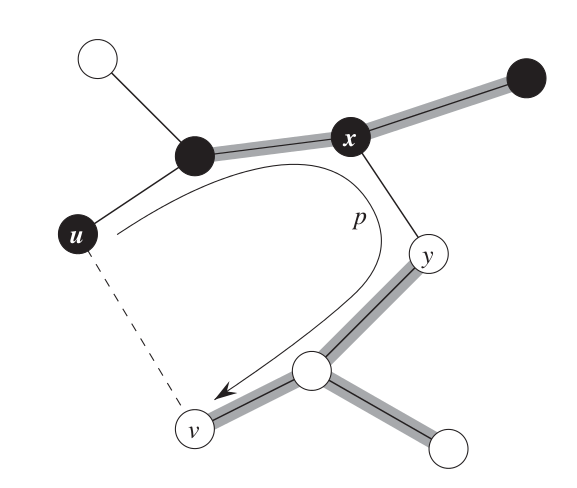
\includegraphics[width=0.5\textwidth]{./safeedge.png} 
\caption{Ilustración de la prueba de la regla la encontrar un borde seguro}
\label{F:MST3}
\end{figure}

De esta manera T' debe ser un árbol de expansión mínima también, además tenemos que A $\subseteq$ T', y A $\subseteq$ T además ($x, y$) $\notin$ A; en consecuencia A$\cup {(u, v)} \subseteq T'$, entonces ($u, v$) es seguro para A.

El ciclo \textbf{while} en las líneas 2-4, del seudocódigo anterior se ejecuta V-1 veces. Inicialmente cuando A =$ \emptyset$, hay V árboles en $G_A = (G,A)$, y cada iteración reduce ese número en 1. Cuando el bosque contiene un solo árbol, el método termina. Ambos algoritmos implementados siguen esta regla, solo que cada uno usa una regla específica para encontrar la borde seguro de la línea 3.

\subsubsection{Clase WeightedEdge}

Para representar un grafo de bordes con peso se procedió a extender la clase graph básica, en una representación de matriz de adyacencia, la cual puede contener bordes con peso en lugar de valores enteros, los cuales están formados por los nodos y su peso. Para esto se creó una clase Edge y WeightedGraph que cuentan con los siguientes métodos:


\begin{table}[h]\center
\begin{tabular}{|l|l|}
\hline
\multicolumn{2}{|c|}{\textbf{API Clase Edge}}                                                                                                            \\ \hline
Edge(int u, int v, float w)    & \begin{tabular}[c]{@{}c@{}}método constructor, inicializa el borde a \\ partir de sus nodos u, v y peso w\end{tabular} \\ \hline
float weight()                 & devuelve el peso del borde                                                                                           \\ \hline
int either()                   & \begin{tabular}[c]{@{}c@{}}devuelve cualquiera de los nodos \\ que conforman el borde\end{tabular}                     \\ \hline
int other(int v)               & devuelve el nodo u                                                                                                      \\ \hline
int compareTo(Edge e)          & compara el peso w con el del borde e                                                                                 \\ \hline
void toString()                & imprime los nodos y el peso del borde                                                                                \\ \hline
Edge\& operator=(const Edge\&) & \begin{tabular}[c]{@{}c@{}}sobrecarga del operador asignación para \\ los objetos Edge\end{tabular}                     \\ \hline
\end{tabular}
\end{table}

\begin{table}[h]\center
\begin{tabular}{|l|l|}
\hline
\multicolumn{2}{|c|}{\textbf{API Clase WeightedGraph}}                                                                                                               \\ \hline
WeightedGraph(int V) & \begin{tabular}[c]{@{}c@{}}método constructor, inicializa y reserva \\ memoria para un grafo de V vértices\end{tabular}                       \\ \hline
int V()              & devuelve el número de vértices del grafo                                                                                                      \\ \hline
int E()              & devuelve el número de bordes del grafo                                                                                                       \\ \hline

void addEdge(Edge e) & \begin{tabular}[c]{@{}c@{}}agrega un objeto edge al grafo y a la \\ lista de adyacencia\end{tabular}                     \\ \hline
\end{tabular}
\end{table}

Cada bolsa de la lista de adyacencia es una lista enlazada, respetando la implementación de los algoritmos de grafos indirectos y directos, cuyo contenido referencia a objetos Edge, o bordes que se conectan a el nodo $v$. Se selecciona esta estructura debido a que logra un código más compacto y limpio, sin embargo conlleva un pequeño precio, cada nodo de la lista de adyacencia, tiene una referencia a un objeto Edge con información redundante. Sin embargo tenemos solo una copia de cada uno. 

El tipo de datos que analizarán los programas tienen la siguiente estructura:\\
\textbf{Grafo TinyEW, de la figura \ref{MST1}:}
\begin{verbatim}
8
16
4 5 0.35
4 7 0.37
5 7 0.28
0 7 0.16
1 5 0.32
0 4 0.38
2 3 0.17
1 7 0.19
0 2 0.26
1 2 0.36
1 3 0.29
2 7 0.34
6 2 0.40
3 6 0.52
6 0 0.58
6 4 0.93
\end{verbatim}
Donde en la primera fila se especifica el número de vértices, en la segunda el número de bordes, y en las siguientes filas se define cada borde, en las cuales primero se muestran los dos nodos que une y el tercer número corresponde a su peso. A este tipo de grafo se le llama Euclidiano, ya que todos sus vértices son puntos que se encuentran en un mismo plano. El objetivo es encontrar el MST de tal tipo de grafo en una cantidad de tiempo razonable. Obteniendo un resultado como el siguiente:
\begin{verbatim}
El MST del grafo anterior es:
0-7 0.16
1-7 0.19
0-2 0.26
2-3 0.17
5-7 0.28
4-5 0.35
6-2 0.40
su peso total es: 1.81
\end{verbatim}

\subsubsection{Algoritmo de Prim}

Este algoritmo es un caso especial del método genérico mostrado en la sección anterior. Tiene la propiedad de que cada borde en el conjunto A siempre forma un solo árbol. Como lo muestra la figura ref3, el árbol empieza de un vértice raiz arbitrario $r$ y crece hasta que se expanda por todos los vértices en V. Cada paso agrega un borde liviano al árbol A, que lo conecta con un vértice aislado, el cual es seguro para A; por lo tanto cuando el algoritmo termina, A forma un árbol de expansión mínima. 

\textbf{Estructuras de datos:} Estas van a representar los vértices en el árbol, las bordes en el árbol, y los bordes que cruzan los cortes, de la siguiente manera:
\begin{itemize}
\item \textit{Vértices en el árbol}: Utilizamos un array booleano indexado llamado marked[ ], donde marked[v] es true si v está en el árbol.
\item \textit{bordes en el árbol}: Se pueden utilizar dos estructuras: una cola llamada mst para almacenar objetos Edge o un array indexado llamado edgeTo[ ] de objetos Edge, donde edgeTo[v] es la borde que conecta v con el árbol.
\item \textit{bordes cruzando un corte}: Utilizamos una cola de prioridad MinPQ que compara bordes por peso.  
\end{itemize}

\begin{figure}[!h]
    \begin{tikzpicture}
        \DrawEJcGraph{}{0/4,0/2,0/6}{7/0}{}{}
        \DrawArrow{xshift=11cm,scale=0.4}
        \DrawEJcGraph{0,7}{0/4,0/2,0/6,5/7}{7/1}{7/0}{xshift=6.7cm}
        \DrawArrow{xshift=24.5cm,scale=0.4}
        \DrawEJcGraph{0,7,1}{0/4,0/6,5/7,1/3}{0/2}{7/0,7/1}{yshift=-3cm}
        \DrawArrow{xshift=11cm,yshift=-6cm,scale=0.4}        
        \DrawEJcGraph{7,0,1,2}{0/4,5/7,2/6}{2/3}{7/0,3/2,0/2}{yshift=-3cm,xshift=6.7cm}
        \DrawArrow{xshift=24.5cm,yshift=-6cm,scale=0.4}
        \DrawEJcGraph{7,0,1,2,3}{0/4,2/6}{5/7}{7/0,3/2,7/1,2/3,0/2}{yshift=-6cm}
        \DrawArrow{xshift=11cm,yshift=-12cm,scale=0.4}
        \DrawEJcGraph{7,0,1,2,3,5}{2/6}{5/4}{7/0,3/2,7/1,2/3,0/2,5/7}{yshift=-6cm,xshift=6.7cm}
        \DrawArrow{xshift=24.5cm,yshift=-12cm,scale=0.4}
        \DrawEJcGraph{7,0,1,2,3,5,4}{}{2/6}{7/0,3/2,7/1,2/3,0/2,5/7,5/4}{yshift=-9cm}
        \DrawArrow{xshift=11cm,yshift=-18cm,scale=0.4}
        \DrawEJcGraph{6,7,0,1,2,3,5,4}{}{}{7/0,3/2,7/1,0/2,5/7,5/4,2/6}{yshift=-9cm,xshift=6.7cm}
    \end{tikzpicture}
    \caption{Algoritmo paso a paso de Prim Eager, bordes en el MST(azul), bordes livianos(rojo grueso), bordes en pq(rojos delgados)}
    \label{MST4}
\end{figure}

Cada vez que agregamos un borde al árbol, agregamos un vértice también. Para mantener un grupo de bordes cruzantes, debemos agregar a una cola de prioridad todos los bordes de ese vertice que van a los vértices que no forman parte del árbol A, usando marked[ ] para identificarlos. Sin embargo debemos hacer algo adicional, todo borde conectado al vértice recién añadido debe marcarse como ineligible, es decir, no sería más un borde cruzante, porque conectaría dos vértices del árbol, haciéndolo cíclico.

Se desarrollaron dos implementaciones del algoritmo de Prim, una en la cual no se eliminan estos bordes ineligibles y se dejan en la cola de prioridad, al cual llamamos $Lazy$ o perezoso, y otro el cual los elimina de la cola llamado $Eager$. 

Para implementar el algoritmo utilizamos un método privado llamado visit(), que agrega un vértice al árbol, marcándolo en marked[ ], y agregando todos los bordes incidentes (que no son ineligibles si es eager) a este vértice en la cola de prioridad. Un ciclo interno del método toma un borde de la cola, y (si no es ineligible) lo agrega al árbol junto con su vértice, actualizando el grupo de bordes cruzantes llamando de nuevo a visit() con el nuevo vértice agregado como argumento. 

Para implementar el Eager Prim, que es más eficiente, ya que selecciona de una forma más rápida los nuevos bordes que se agregan al árbol A, necesitamos mantener en la cola de prioridad solo un borde por cada vértice $v$ que no esté en A: El mínimo borde, o el más liviano. Los demás se convierten en ineligibles.

En este algoritmo se reemplazan las estructuras de datos marked[ ] y mst[ ] en LazyPrim por dos arrays indexados edgeTo[ ] y distTo[ ], que tienen las siguientes propiedades:

\begin{itemize}
\item Si $v$ no está en el árbol pero tiene al menos un borde conectado a este, entonces edgeTo[v] es el mínimo borde conectando v a el árbol, y distTo[v] es el peso de ese borde.
\item Todos esos vértices v son mantenidos en la cola de prioridad indexada, como un índice v asociado a ese borde.
\end{itemize} 
La mínima clave o $key$ en la cola de prioridad, es el peso del borde liviano, y su vértice asociado v, es el siguiente que se agregará a A. La estructura marked[ ] no es necesaria, ya que la condición !marked[v] es equivalente a la condición distTo[v]=$\infty$.   

\subsubsection{Algoritmo de Kruskal}
Este algoritmo encuentra un borde seguro para agregar al bosque en crecimiento (MST), tomando de todos los que conectan dos árboles cualquiera en el bosque, el de menor peso. Sea $C_1$ y $C_2$ estos dos árboles cualquiera, conectados por ($u, v$), y ya que este debe ser una borde liviano y además conecta a $C_1$ a otro árbol, implica que $(u, v)$ es seguro para $C_1$. 

Empezamos con un bosque degenerado de V vértices individuales y realizamos una operación de combinación de parejas de árboles por medio de bordes livianos, hasta que quede un solo árbol: el MST.

La figura \ref{MST5} ilustra paso por paso un ejemplo de la operación de Kruskal sobre el grafo TinyEW, cuyas aristas se muestran ordenas por peso a continuación, y donde los vértices rojos representan cortes definidos por vértices conectados a una de las aristas de los vértices rojos: 

\begin{verbatim}
0-7 0.16 -arista del MST (azul)
2-3 0.17 -arista del MST (azul)
1-7 0.19 -arista del MST (azul)
0-2 0.26 -arista del MST (azul)
5-7 0.28 -arista del MST (azul)
1-3 0.29 -arista obsoleta (forma un ciclo) (negra) 
1-5 0.32 -arista obsoleta (forma un ciclo) (negra)
2-7 0.34 -arista obsoleta (forma un ciclo) (negra)
4-5 0.35 -arista del MST (azul)
1-2 0.36 -arista obsoleta (forma un ciclo) (negra)
4-7 0.37 -arista obsoleta (forma un ciclo) (negra)
0-4 0.38 -arista obsoleta (forma un ciclo) (negra)
6-2 0.40 -arista del MST (azul)
3-6 0.52 -arista obsoleta (forma un ciclo) (negra)
6-0 0.58 -arista obsoleta (forma un ciclo) (negra)
6-4 0.93 -arista obsoleta (forma un ciclo) (negra)
\end{verbatim}

\begin{figure}[!h]
    \begin{tikzpicture}
        \DrawEJcGraph{}{}{}{}{}
        \DrawArrow{xshift=11cm,scale=0.4}
        \DrawEJcGraph{0}{}{7/0}{}{xshift=6.7cm}
        \DrawArrow{xshift=24.5cm,scale=0.4}
        \DrawEJcGraph{2}{}{3/2}{7/0}{yshift=-3cm}
        \DrawArrow{xshift=11cm,yshift=-6cm,scale=0.4}        
        \DrawEJcGraph{7,0}{}{7/1}{7/0,3/2}{yshift=-3cm,xshift=6.7cm}
        \DrawArrow{xshift=24.5cm,yshift=-6cm,scale=0.4}
        \DrawEJcGraph{7,0,1}{}{0/2}{7/0,3/2,7/1}{yshift=-6cm}
        \DrawArrow{xshift=11cm,yshift=-12cm,scale=0.4}
        \DrawEJcGraph{5}{}{5/7}{7/0,3/2,7/1,0/2}{yshift=-6cm,xshift=6.7cm}
        \DrawArrow{xshift=24.5cm,yshift=-12cm,scale=0.4}
        \DrawEJcGraph{5,7,1,0,2,3}{}{5/4}{7/0,3/2,7/1,0/2,5/7}{yshift=-9cm}
        \DrawArrow{xshift=11cm,yshift=-18cm,scale=0.4}
        \DrawEJcGraph{6}{}{2/6}{7/0,3/2,7/1,0/2,5/7,5/4}{yshift=-9cm,xshift=6.7cm}
    \end{tikzpicture}
    \caption{Algoritmo paso a paso de Kruskal}
    \label{MST5}
\end{figure}

\newpage
\subsection{Algoritmos para la b\'usqueda de la ruta m\'as corta}
Una de las inc\'ognitas m\'as importantes que tiene en el procesamiento de algortmo es: ¿Se puede encontrar un camino \'optimo entre dos v\'ertices del grafo?. La importancia de este problema se puede observar en fen\'omenos tecnol\'ogicos como el ruteo de paquetes en las redes de computadoras. 

La definici\'on del problema es que dado un grafo dirigido con pesos \textit{G = (V,E)}, con una funci\'on de pesos \textit{w : E $\longrightarrow \mathbb{R}$} que mapea los enlaces a valores reales de peso. El peso \textit{w(p)} de un path \textit{p = (v0,...,vk)} es la suma de los pesos de sus enlaces constituyentes. De este modo el path m\'as corto de un v\'ertice u a un v\'ertice v se define como:

INSERTAR ECUACION

Existen dos fen\'omenos importantes que pueden suceder cuano se trata con grafos:
\begin{itemize}
    \item \textit{Enlaces Negativos}
    \item \textit{Ciclos}
\end{itemize}

Con respecto a los enlaces negativos, el problema principal radica en que exista un ciclo de peso negativo (que la suma de los bordes que forman el ciclo sea negativa), ya que si esto ocurre, entonces los paths m\'as cortos no est\'an bien definidos. Esto es debido a que ning\'un camino desde s hasta cualquiera de los nodos en el ciclo puede ser tomado como el m\'as corto.

\subsubsection{Algoritmo de Bellman-Ford}
El algoritmo de Bellman-Ford resuelve el problema del camino m\'as corto, para el caso general en el cual los pesos pueden tomar valores negativos. \'Este propone que dado un grafo dirigido con peso, es posible encontrar un path entre cualquier par de nodos que cumpla con la condici\'on de ser el camino m\'as corto, siempre y cuando no existan ciclos negativos.

El algoritmo se lleva a cabo relajando los enlaces de manera progresiva, disminuyendo un estimado de la distancia a un v\'ertice dado desde la fuente. El pseudoc\'odigo que describe al Bellman-Ford es el propuesto en el algoritmo \ref{Bellman-Ford}

\begin{algorithm}
\caption{Pseudocodigo Bellman Ford}
\label{Bellman-Ford}
\begin{algorithmic}
\Procedure{BellmanFord}{G}
    \ForAll{i = 1 \textbf{to} G.V - 1}
        \ForAll{edge $\in$ G}
            \State Relax(u,v,w)
        \EndFor
    \EndFor
    \ForAll{edge $\in$ G}
        \If{v.d $\geq$ u.d + w(u,v)}
            \State \textbf{return} FALSE
        \EndIf
    \EndFor
\EndProcedure
\end{algorithmic}
\end{algorithm}

Como se observa en el algoritmo se llama a un procedimiento denominado relajaci\'on. En este procedimiento se itera sobre los enlaces para definir distintos pesos para cada uno y se itera hasta saber el valor \'optimo del camino hasta el v\'ertice. El algoritmo corre en un tiempo polinomial de O(VE).

\subsubsection{Algoritmo de Djikstra}
El algoritmo de Djikstra es utilizado para resolver el problema del camino m\'as corto en grafos dirigidos con valores de peso positivo. El algoritmo mantiene un conjunto de v\'ertices a los cuales ya se les ha determinado el camino m\'as corto desde el origen. El algoritmo selecciona de manerar repetitiva el v\'ertice con el estimado m\'as bajo, para esto se hace uso de una cola de prioridad. El algoritmo b\'asico es el \ref{Djikstra}.

\begin{algorithm}
\caption{Algoritmo de Djikstra}
\label{Djikstra}
\begin{algorithmic}
\Procedure{Djikstra}{G,w,s}
    \State S = 0
    \State Q = G.V
    \While{Q $\neq$ 0}
        \State u = Min(Q)
        \State S = S U {u}
        \ForAll{vertex $\in$ adj[u]}
            \State Relax(u,v,w)
        \EndFor
    \EndWhile    
\EndProcedure
\end{algorithmic}
\end{algorithm}

El algoritmo relaja los enlaces de manera que pueda ir determinando el valor m\'as bajo de la cola de prioridad. La cola de prioridad es sumamente importante en la implementaci\'on debido a que permite obtener el valor m\'inimo del sistema que ser\'a elegido como el camino \'optimo hacia cierto v\'ertice.

\end{document}
